\documentclass[]{article}
\usepackage{lmodern}
\usepackage{amssymb,amsmath}
\usepackage{ifxetex,ifluatex}
\usepackage{fixltx2e} % provides \textsubscript
\ifnum 0\ifxetex 1\fi\ifluatex 1\fi=0 % if pdftex
  \usepackage[T1]{fontenc}
  \usepackage[utf8]{inputenc}
\else % if luatex or xelatex
  \ifxetex
    \usepackage{mathspec}
  \else
    \usepackage{fontspec}
  \fi
  \defaultfontfeatures{Ligatures=TeX,Scale=MatchLowercase}
\fi
% use upquote if available, for straight quotes in verbatim environments
\IfFileExists{upquote.sty}{\usepackage{upquote}}{}
% use microtype if available
\IfFileExists{microtype.sty}{%
\usepackage{microtype}
\UseMicrotypeSet[protrusion]{basicmath} % disable protrusion for tt fonts
}{}
\usepackage[margin=1in]{geometry}
\usepackage{hyperref}
\hypersetup{unicode=true,
            pdfborder={0 0 0},
            breaklinks=true}
\urlstyle{same}  % don't use monospace font for urls
\usepackage{color}
\usepackage{fancyvrb}
\newcommand{\VerbBar}{|}
\newcommand{\VERB}{\Verb[commandchars=\\\{\}]}
\DefineVerbatimEnvironment{Highlighting}{Verbatim}{commandchars=\\\{\}}
% Add ',fontsize=\small' for more characters per line
\usepackage{framed}
\definecolor{shadecolor}{RGB}{248,248,248}
\newenvironment{Shaded}{\begin{snugshade}}{\end{snugshade}}
\newcommand{\KeywordTok}[1]{\textcolor[rgb]{0.13,0.29,0.53}{\textbf{#1}}}
\newcommand{\DataTypeTok}[1]{\textcolor[rgb]{0.13,0.29,0.53}{#1}}
\newcommand{\DecValTok}[1]{\textcolor[rgb]{0.00,0.00,0.81}{#1}}
\newcommand{\BaseNTok}[1]{\textcolor[rgb]{0.00,0.00,0.81}{#1}}
\newcommand{\FloatTok}[1]{\textcolor[rgb]{0.00,0.00,0.81}{#1}}
\newcommand{\ConstantTok}[1]{\textcolor[rgb]{0.00,0.00,0.00}{#1}}
\newcommand{\CharTok}[1]{\textcolor[rgb]{0.31,0.60,0.02}{#1}}
\newcommand{\SpecialCharTok}[1]{\textcolor[rgb]{0.00,0.00,0.00}{#1}}
\newcommand{\StringTok}[1]{\textcolor[rgb]{0.31,0.60,0.02}{#1}}
\newcommand{\VerbatimStringTok}[1]{\textcolor[rgb]{0.31,0.60,0.02}{#1}}
\newcommand{\SpecialStringTok}[1]{\textcolor[rgb]{0.31,0.60,0.02}{#1}}
\newcommand{\ImportTok}[1]{#1}
\newcommand{\CommentTok}[1]{\textcolor[rgb]{0.56,0.35,0.01}{\textit{#1}}}
\newcommand{\DocumentationTok}[1]{\textcolor[rgb]{0.56,0.35,0.01}{\textbf{\textit{#1}}}}
\newcommand{\AnnotationTok}[1]{\textcolor[rgb]{0.56,0.35,0.01}{\textbf{\textit{#1}}}}
\newcommand{\CommentVarTok}[1]{\textcolor[rgb]{0.56,0.35,0.01}{\textbf{\textit{#1}}}}
\newcommand{\OtherTok}[1]{\textcolor[rgb]{0.56,0.35,0.01}{#1}}
\newcommand{\FunctionTok}[1]{\textcolor[rgb]{0.00,0.00,0.00}{#1}}
\newcommand{\VariableTok}[1]{\textcolor[rgb]{0.00,0.00,0.00}{#1}}
\newcommand{\ControlFlowTok}[1]{\textcolor[rgb]{0.13,0.29,0.53}{\textbf{#1}}}
\newcommand{\OperatorTok}[1]{\textcolor[rgb]{0.81,0.36,0.00}{\textbf{#1}}}
\newcommand{\BuiltInTok}[1]{#1}
\newcommand{\ExtensionTok}[1]{#1}
\newcommand{\PreprocessorTok}[1]{\textcolor[rgb]{0.56,0.35,0.01}{\textit{#1}}}
\newcommand{\AttributeTok}[1]{\textcolor[rgb]{0.77,0.63,0.00}{#1}}
\newcommand{\RegionMarkerTok}[1]{#1}
\newcommand{\InformationTok}[1]{\textcolor[rgb]{0.56,0.35,0.01}{\textbf{\textit{#1}}}}
\newcommand{\WarningTok}[1]{\textcolor[rgb]{0.56,0.35,0.01}{\textbf{\textit{#1}}}}
\newcommand{\AlertTok}[1]{\textcolor[rgb]{0.94,0.16,0.16}{#1}}
\newcommand{\ErrorTok}[1]{\textcolor[rgb]{0.64,0.00,0.00}{\textbf{#1}}}
\newcommand{\NormalTok}[1]{#1}
\usepackage{graphicx,grffile}
\makeatletter
\def\maxwidth{\ifdim\Gin@nat@width>\linewidth\linewidth\else\Gin@nat@width\fi}
\def\maxheight{\ifdim\Gin@nat@height>\textheight\textheight\else\Gin@nat@height\fi}
\makeatother
% Scale images if necessary, so that they will not overflow the page
% margins by default, and it is still possible to overwrite the defaults
% using explicit options in \includegraphics[width, height, ...]{}
\setkeys{Gin}{width=\maxwidth,height=\maxheight,keepaspectratio}
\IfFileExists{parskip.sty}{%
\usepackage{parskip}
}{% else
\setlength{\parindent}{0pt}
\setlength{\parskip}{6pt plus 2pt minus 1pt}
}
\setlength{\emergencystretch}{3em}  % prevent overfull lines
\providecommand{\tightlist}{%
  \setlength{\itemsep}{0pt}\setlength{\parskip}{0pt}}
\setcounter{secnumdepth}{0}
% Redefines (sub)paragraphs to behave more like sections
\ifx\paragraph\undefined\else
\let\oldparagraph\paragraph
\renewcommand{\paragraph}[1]{\oldparagraph{#1}\mbox{}}
\fi
\ifx\subparagraph\undefined\else
\let\oldsubparagraph\subparagraph
\renewcommand{\subparagraph}[1]{\oldsubparagraph{#1}\mbox{}}
\fi

%%% Use protect on footnotes to avoid problems with footnotes in titles
\let\rmarkdownfootnote\footnote%
\def\footnote{\protect\rmarkdownfootnote}

%%% Change title format to be more compact
\usepackage{titling}

% Create subtitle command for use in maketitle
\newcommand{\subtitle}[1]{
  \posttitle{
    \begin{center}\large#1\end{center}
    }
}

\setlength{\droptitle}{-2em}
  \title{}
  \pretitle{\vspace{\droptitle}}
  \posttitle{}
  \author{}
  \preauthor{}\postauthor{}
  \date{}
  \predate{}\postdate{}


\begin{document}

\section{R Statistics Demo - Model
Comparison}\label{r-statistics-demo---model-comparison}

Goal of demo is to accurately predict Sparks case pick volume by
hour/day.

Dependent variable: boxes received

Independent variables:

\begin{itemize}
\tightlist
\item
  Hour of Day
\item
  Workday of Month - business day of month (weekends are excluded)
\item
  Week of Month - week number of month
\item
  Week Day - day number of week (2=mon, 6=fri)
\item
  Day of Month - day of month (weekends are included)
\item
  Month of Year - Month number of year (1-12)
\item
  Year
\item
  Before Vacation - Is this a day before holiday? (1=yes, 0=no)
\item
  After Vacation - Is this a day after a holiday? (1=yes, 0=no)
\item
  Before Chirstmas - Is this the day before Christmas? (1=yes, 0=no)
\item
  After Christmas - Is this the day after Christmas? (1=yes, 0=no)
\end{itemize}

The following demo will test 5 predictive models:

\begin{enumerate}
\def\labelenumi{\arabic{enumi}.}
\tightlist
\item
  Linear Regression
\item
  Decision Tree
\item
  Random Forest
\item
  Neural Net
\item
  Boosted Tree
\end{enumerate}

The measuring statistic will be root mean squared error (RMSE).

\begin{Shaded}
\begin{Highlighting}[]
\NormalTok{knitr}\OperatorTok{::}\NormalTok{opts_chunk}\OperatorTok{$}\KeywordTok{set}\NormalTok{(}\DataTypeTok{message =} \OtherTok{FALSE}\NormalTok{)}
\NormalTok{packages <-}\StringTok{ }\KeywordTok{c}\NormalTok{(}\StringTok{'useful'}\NormalTok{, }\StringTok{'coefplot'}\NormalTok{, }\StringTok{'xgboost'}\NormalTok{, }\StringTok{'here'}\NormalTok{, }\StringTok{'magrittr'}\NormalTok{, }\StringTok{'dygraphs'}\NormalTok{, }\StringTok{'dplyr'}\NormalTok{, }\StringTok{'RMySQL'}\NormalTok{, }\StringTok{'caret'}\NormalTok{, }\StringTok{'purrr'}\NormalTok{, }\StringTok{'randomForest'}\NormalTok{, }\StringTok{'rpart'}\NormalTok{, }\StringTok{'neuralnet'}\NormalTok{, }\StringTok{'tictoc'}\NormalTok{, }\StringTok{'tinytex'}\NormalTok{, }\StringTok{'DT'}\NormalTok{)}
\NormalTok{purrr}\OperatorTok{::}\KeywordTok{walk}\NormalTok{(packages, library, }\DataTypeTok{character.only =} \OtherTok{TRUE}\NormalTok{)}
\CommentTok{#lapply( dbListConnections( dbDriver( drv = "MySQL")), dbDisconnect)}
\CommentTok{#dev}
\CommentTok{#mychannel <- dbConnect(MySQL(), user="bentley", pass="dave41", host="127.0.0.1")}

\CommentTok{#NY Server Prod}
\NormalTok{mychannel <-}\StringTok{ }\KeywordTok{dbConnect}\NormalTok{(}\KeywordTok{MySQL}\NormalTok{(), }\DataTypeTok{user=}\StringTok{"root"}\NormalTok{, }\DataTypeTok{pass=}\StringTok{"dave41"}\NormalTok{, }\DataTypeTok{host=}\StringTok{"127.0.0.1"}\NormalTok{)}

\CommentTok{#Google Prod}
\CommentTok{#mychannel <- dbConnect(MySQL(), user="bentley", pass="dave41", host="104.154.153.225")}

\NormalTok{query <-}\StringTok{ }\ControlFlowTok{function}\NormalTok{(...) }\KeywordTok{dbGetQuery}\NormalTok{(mychannel, ...)}
\end{Highlighting}
\end{Shaded}

\section{Load historical data}\label{load-historical-data}

\begin{Shaded}
\begin{Highlighting}[]
\CommentTok{# var_whse <- 3}
\CommentTok{# var_build <- 2}
\CommentTok{# }
\CommentTok{# sqlquery <- paste("SELECT }
\CommentTok{#                   CASE}
\CommentTok{#                   WHEN predicted_availhour < 6 THEN 6}
\CommentTok{#                   WHEN predicted_availhour > 16 THEN 16}
\CommentTok{#                   ELSE predicted_availhour}
\CommentTok{#                   }\RegionMarkerTok{END}\CommentTok{ AS HOUR,}
\CommentTok{#                   workday_workday AS WORKDAY,}
\CommentTok{#                   workday_weekofmon AS MONTHWEEK,}
\CommentTok{#                   workday_weekday AS WEEKDAY,}
\CommentTok{#                   workday_dayofmon AS MONTHDAY,}
\CommentTok{#                   workday_month AS MONTH,}
\CommentTok{#                   YEAR(predicted_availdate) as YEAR,}
\CommentTok{#                   workday_befvac AS BEFVAC,}
\CommentTok{#                   workday_aftvac AS AFTVAC,}
\CommentTok{#                   workday_befchrist AS BEFCHR,}
\CommentTok{#                   workday_aftchrist AS AFTCHR,}
\CommentTok{#                   SUM(CASE}
\CommentTok{#                   WHEN}
\CommentTok{#                   hist_twoday = 1}
\CommentTok{#                   AND predicted_availhour < 6}
\CommentTok{#                   THEN}
\CommentTok{#                   1}
\CommentTok{#                   ELSE 1}
\CommentTok{#                   }\RegionMarkerTok{END}\CommentTok{) AS BOXES}
\CommentTok{#                   FROM}
\CommentTok{#                   printvis.hist_casevol}
\CommentTok{#                   JOIN}
\CommentTok{#                   printvis.workdayofweek ON predicted_availdate = workday_date}
\CommentTok{#                   WHERE }
\CommentTok{#                   hist_whse = ",var_whse," and hist_build = ",var_build," }
\CommentTok{#                   AND hist_equip = 'PALLETJACK'}
\CommentTok{#                   AND cutoff_group NOT IN ('TRUCK' , 'COLGATE')}
\CommentTok{#                   AND predicted_availhour BETWEEN 7 AND 16}
\CommentTok{#                   GROUP BY predicted_availdate , hist_equip, }
\CommentTok{#                   CASE}
\CommentTok{#                   WHEN predicted_availhour < 6 THEN 6}
\CommentTok{#                   WHEN predicted_availhour > 16 THEN 16}
\CommentTok{#                   ELSE predicted_availhour}
\CommentTok{#                   }\RegionMarkerTok{END}
\CommentTok{#                   ORDER BY predicted_availdate , CASE}
\CommentTok{#                   WHEN predicted_availhour < 6 THEN 6}
\CommentTok{#                   WHEN predicted_availhour > 16 THEN 16}
\CommentTok{#                   ELSE predicted_availhour}
\CommentTok{#                   }\RegionMarkerTok{END}\CommentTok{", sep = "")}
\CommentTok{# data <- query(sqlquery)}
\CommentTok{# }
\CommentTok{# DT::datatable(head(data))}
\CommentTok{# head(data)}
\end{Highlighting}
\end{Shaded}

\section{Set seed and determine training and test
data}\label{set-seed-and-determine-training-and-test-data}

\begin{Shaded}
\begin{Highlighting}[]
\CommentTok{# set.seed(222)}
\CommentTok{# trainIndex <- createDataPartition(data$BOXES, }
\CommentTok{#                                   p = .75, }
\CommentTok{#                                   list = FALSE, }
\CommentTok{#                                   times = 1)}
\CommentTok{# }
\CommentTok{# dataTrain <- data[ trainIndex,]}
\CommentTok{# dataTest  <- data[-trainIndex,]}
\CommentTok{# }
\CommentTok{# DT::datatable(head(dataTrain))}
\CommentTok{# DT::datatable(head(dataTest))}
\CommentTok{# }
\CommentTok{# }
\CommentTok{# data_formula_boxes <- BOXES ~ HOUR + WORKDAY + MONTHWEEK + WEEKDAY + MONTHDAY + MONTH + YEAR + BEFVAC + AFTVAC + BEFCHR + AFTCHR}
\CommentTok{# }
\CommentTok{# #boxes data training}
\CommentTok{# dataX_Train_box <- build.x(data_formula_boxes, data=dataTrain,}
\CommentTok{#                        contrasts=FALSE,}
\CommentTok{#                        sparse=TRUE)}
\CommentTok{# dataY_Train_box <- build.y(data_formula_boxes,data=dataTrain) }
\CommentTok{# }
\CommentTok{# dataX_Test_box <- build.x(data_formula_boxes, data=dataTest,}
\CommentTok{#                       contrasts=FALSE,}
\CommentTok{#                       sparse=TRUE)}
\CommentTok{# dataY_Test_box <- build.y(data_formula_boxes,data=dataTest)}
\CommentTok{# }
\CommentTok{# xgTrain_box <- xgb.DMatrix(data=dataX_Train_box,}
\CommentTok{#                        label=dataY_Train_box)}
\CommentTok{# }
\CommentTok{# xgVal_box <- xgb.DMatrix(data=dataX_Test_box,}
\CommentTok{#                      label=dataY_Test_box)}
\end{Highlighting}
\end{Shaded}

\section{Create the Linear regression
model}\label{create-the-linear-regression-model}

\begin{figure}
\centering
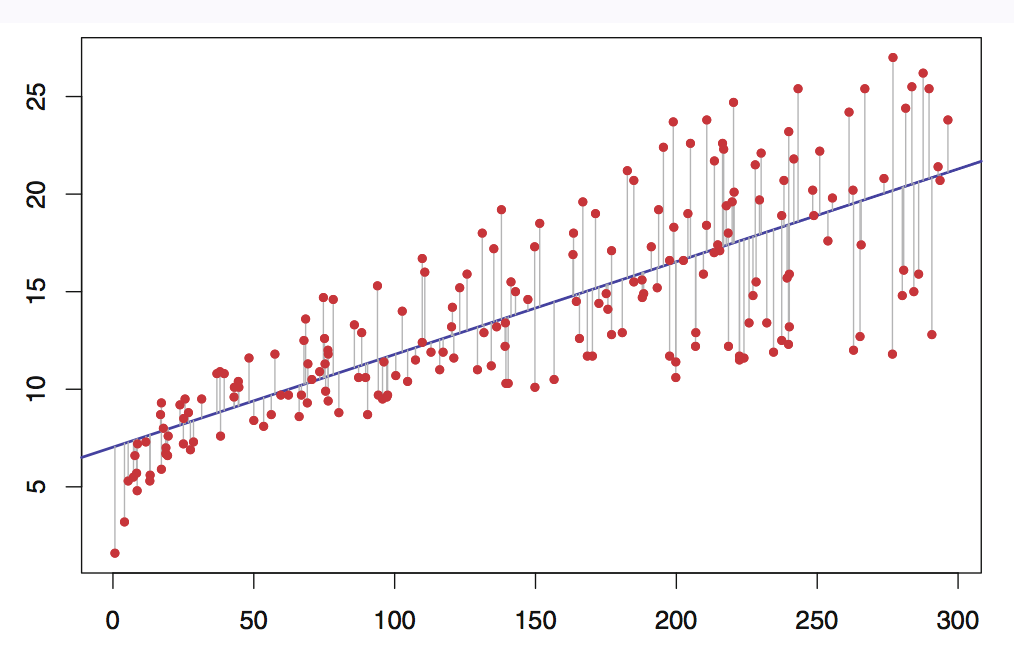
\includegraphics{regression.png}
\caption{Linear Regression - Least Squares}
\end{figure}

\section{Create the decision tree
model}\label{create-the-decision-tree-model}

\begin{Shaded}
\begin{Highlighting}[]
\CommentTok{# model.dt <- rpart(data_formula_boxes, method = "anova", data=dataTrain)}
\CommentTok{# prediction.dt <- predict(model.dt, newdata = dataTest)}
\CommentTok{# rmse.dt <- sqrt(mean((dataTest$BOXES-prediction.dt)^2))}
\CommentTok{# rmse.dt}
\CommentTok{# plot(dataTest$BOXES,prediction.dt,col='blue',main='Real vs predicted Decision Tree',pch=18, cex=0.7)}
\CommentTok{# abline(0,1,lwd=2)}
\end{Highlighting}
\end{Shaded}

\section{Create the random forest
model}\label{create-the-random-forest-model}

\begin{Shaded}
\begin{Highlighting}[]
\CommentTok{# dataTrain_fac <- dataTrain %>% mutate_if(is.character, as.factor)}
\CommentTok{# dataTest_fac <- dataTest %>% mutate_if(is.character, as.factor)}
\CommentTok{# model.rf <- randomForest(data_formula_boxes, data = dataTrain_fac)}
\CommentTok{# prediction.rf <- predict(model.rf, newdata = dataTest_fac)}
\CommentTok{# rmse.rf <- sqrt(mean((dataTest_fac$BOXES-prediction.rf)^2))}
\CommentTok{# rmse.rf}
\CommentTok{# plot(dataTest$BOXES,prediction.rf,col='blue',main='Real vs predicted Random Forest',pch=18, cex=0.7)}
\CommentTok{# abline(0,1,lwd=2)}
\end{Highlighting}
\end{Shaded}

\section{Create the neural net mode}\label{create-the-neural-net-mode}

\begin{Shaded}
\begin{Highlighting}[]
\CommentTok{# library('neuralnet')}
\CommentTok{# }
\CommentTok{# maxs <- apply(dataTrain, 2, max)}
\CommentTok{# mins <- apply(dataTrain, 2, min)}
\CommentTok{# scaled_train <- as.data.frame(scale(dataTrain, center = mins, scale = maxs - mins))}
\CommentTok{# scaled_test <- as.data.frame(scale(dataTest, center = mins, scale = maxs - mins))}
\CommentTok{# n <- names(scaled_train)}
\CommentTok{# f <- as.formula(paste("BOXES ~", paste(n[!n %in% "BOXES"], collapse = " + ")))}
\CommentTok{# }
\CommentTok{# nn <- neuralnet(f,data=scaled_train,hidden=c(8,4),linear.output=F)}
\CommentTok{# pr.nn <- compute(nn,scaled_test[,0:11])}
\CommentTok{# pr.nn_ <- pr.nn$net.result*(max(data$BOXES)-min(data$BOXES))+min(data$BOXES)}
\CommentTok{# test.r <- (scaled_test$BOXES)*(max(data$BOXES)-min(data$BOXES))+min(data$BOXES)}
\CommentTok{# rmse.nn <- sqrt(mean((dataTest$BOXES-pr.nn_)^2))}
\CommentTok{# rmse.nn}
\CommentTok{# }
\CommentTok{#  plot(dataTest$BOXES,pr.nn_,col='blue',main='Real vs predicted Neural Net',pch=18, cex=0.7)}
\CommentTok{#  abline(0,1,lwd=2)}
\end{Highlighting}
\end{Shaded}

\section{Create the boosted random forest
model}\label{create-the-boosted-random-forest-model}

\begin{Shaded}
\begin{Highlighting}[]
\CommentTok{# tic()}
\CommentTok{# model.xgb <- xgb.train(data=xgTrain_box, objective='reg:linear', eval_metric='rmse', booster='gbtree', watchlist = list(train=xgTrain_box, validate=xgVal_box),}
\CommentTok{#                   early_stopping_rounds=100, nrounds = 100000, num_parallel_tree=20, print_every_n = 20, nthread=8,eta = .1, max_depth = 7)}
\CommentTok{# toc()}
\CommentTok{# dataTest.xgb <- build.x(data_formula_boxes, data=dataTest, contrasts = FALSE, sparse = TRUE)}
\CommentTok{# }
\CommentTok{# prediction.xgb <- predict(model.xgb, newdata = dataTest.xgb)}
\CommentTok{# plot(dataTest$BOXES,prediction.xgb,col='blue',main='Real vs predicted Boosted Forest',pch=18, cex=0.7)}
\CommentTok{#  abline(0,1,lwd=2)}
\end{Highlighting}
\end{Shaded}


\end{document}
